%!TEX program = xelatex
\documentclass[9pt, compress]{beamer}
\usetheme[titleprogressbar]{m}

\usepackage{array}
\usepackage{tabu}
\usepackage{longtable} %tabu needs this to be loaded.
\usepackage{lipsum}

\usepackage{rotating}

\usepackage{color}
\usepackage{xcolor}
\usepackage{listings}
\usepackage{sectsty}
\usepackage{caption}


\DeclareCaptionFont{white}{\color{white}}
\DeclareCaptionFormat{listing}{\colorbox{gray}{\parbox{\dimexpr\textwidth-1.72\fboxsep\relax}{#1#2#3}}}
\captionsetup[lstlisting]{format=listing,labelfont=white,textfont=white,margin=0pt}
\lstset{language=C,
	basicstyle=\footnotesize,
	keepspaces=true,
	tabsize=4,               
	frame=single,                           % Single frame around code
	rulecolor=\color{black},
	captionpos=b,
	showstringspaces=false,	
	abovecaptionskip=-0.9pt,
	xleftmargin=3.4pt,
	xrightmargin=2.6pt,
	breaklines=true,
	postbreak=\raisebox{0ex}[0ex][0ex]{\ensuremath{\color{black}\hookrightarrow\space}},
	xleftmargin=3.2pt,
	escapechar=\&,
	literate={а}{{\selectfont\char224}}1
	{~}{{\textasciitilde}}1
	{б}{{\selectfont\char225}}1
	{в}{{\selectfont\char226}}1
	{г}{{\selectfont\char227}}1
	{д}{{\selectfont\char228}}1
	{е}{{\selectfont\char229}}1
	{ё}{{\"e}}1
	{ж}{{\selectfont\char230}}1
	{з}{{\selectfont\char231}}1
	{и}{{\selectfont\char232}}1
	{й}{{\selectfont\char233}}1
	{к}{{\selectfont\char234}}1
	{л}{{\selectfont\char235}}1
	{м}{{\selectfont\char236}}1
	{н}{{\selectfont\char237}}1
	{о}{{\selectfont\char238}}1
	{п}{{\selectfont\char239}}1
	{р}{{\selectfont\char240}}1
	{с}{{\selectfont\char241}}1
	{т}{{\selectfont\char242}}1
	{у}{{\selectfont\char243}}1
	{ф}{{\selectfont\char244}}1
	{х}{{\selectfont\char245}}1
	{ц}{{\selectfont\char246}}1
	{ч}{{\selectfont\char247}}1
	{ш}{{\selectfont\char248}}1
	{щ}{{\selectfont\char249}}1
	{ъ}{{\selectfont\char250}}1
	{ы}{{\selectfont\char251}}1
	{ь}{{\selectfont\char252}}1
	{э}{{\selectfont\char253}}1
	{ю}{{\selectfont\char254}}1
	{я}{{\selectfont\char255}}1
	{А}{{\selectfont\char192}}1
	{Б}{{\selectfont\char193}}1
	{В}{{\selectfont\char194}}1
	{Г}{{\selectfont\char195}}1
	{Д}{{\selectfont\char196}}1
	{Е}{{\selectfont\char197}}1
	{Ё}{{\"E}}1
	{Ж}{{\selectfont\char198}}1
	{З}{{\selectfont\char199}}1
	{И}{{\selectfont\char200}}1
	{Й}{{\selectfont\char201}}1
	{К}{{\selectfont\char202}}1
	{Л}{{\selectfont\char203}}1
	{М}{{\selectfont\char204}}1
	{Н}{{\selectfont\char205}}1
	{О}{{\selectfont\char206}}1
	{П}{{\selectfont\char207}}1
	{Р}{{\selectfont\char208}}1
	{С}{{\selectfont\char209}}1
	{Т}{{\selectfont\char210}}1
	{У}{{\selectfont\char211}}1
	{Ф}{{\selectfont\char212}}1
	{Х}{{\selectfont\char213}}1
	{Ц}{{\selectfont\char214}}1
	{Ч}{{\selectfont\char215}}1
	{Ш}{{\selectfont\char216}}1
	{Щ}{{\selectfont\char217}}1
	{Ъ}{{\selectfont\char218}}1
	{Ы}{{\selectfont\char219}}1
	{Ь}{{\selectfont\char220}}1
	{Э}{{\selectfont\char221}}1
	{Ю}{{\selectfont\char222}}1
	{Я}{{\selectfont\char223}}1,
	extendedchars=true
}

%галочка
\usepackage{amssymb}% http://ctan.org/pkg/amssymb
\usepackage{pifont}% http://ctan.org/pkg/pifont
\newcommand{\cmark}{\ding{52}}%
\newcommand{\xmark}{\ding{56}}

\usepackage{booktabs}  
\usepackage[scale=2]{ccicons}
\usepackage{minted}
\usepgfplotslibrary{dateplot}
\usemintedstyle{trac}
\author{Студент: \textbf{Д.В. Круминьш}\\ 
	Группа: \textbf{13541/3}\\ \\
	Преподаватель: \textbf{И.А. Малышев} } 
\title{Отчет о лабораторной работе №1}
\subtitle{Курс: \textbf{Администрирование компьютерных сетей}\\
Тема: \textbf{Виртуальное макетирование компьютерных сетей}}
%\logo{123}
\institute{Санкт-Петербургский политехнический университет Петра Великого}
\date{ }
%\subject{}
%\setbeamercovered{transparent}
%\setbeamertemplate{navigation symbols}{}
\begin{document}
	\maketitle
%%	\begin{frame}
%%		\frametitle{Оглавление}
%%		\tableofcontents{}
%	\end{frame}
\begin{frame}
\frametitle{Цели работы}
\begin{enumerate}
\item Изучить технологию виртуального макетирования компьютерных сетей в среде VMware Workstation.
\item Разработать и настроить полунатуральный эмулятор компьютерной сети.
\end{enumerate}
\end{frame}

\begin{frame}
\frametitle{Сведения о системе}
Работа производилась на реальной системе, со следующими характеристиками:
\tabulinesep = 1mm
\begin{longtabu} to \textwidth {|X[10, c , m ] |X[25, c , m ] | }\firsthline\hline

\textbf{Элемент}&\textbf{Значение}\\ \hline \endfirsthead
	
Имя ОС&Майкрософт Windows 10 Pro (Registered Trademark)\\ \hline
Версия&10.0.16299 Сборка 16299\\ \hline
Установленная оперативная память (RAM) &16,00 ГБ\\ \hline
Процессор&Intel(R) Core(TM) i5-7300HQ CPU @ 2.50GHz, 2496 МГц, ядер: 4, логических процессоров: 4\\ \hline
\end{longtabu}
Для выполнения работы использовалась \textbf{VMware Workstation 12 pro (12.5.7 build-5813279)}
\end{frame}

\begin{frame}
\frametitle{Макет разрабатываемой сети}
\begin{center}  
	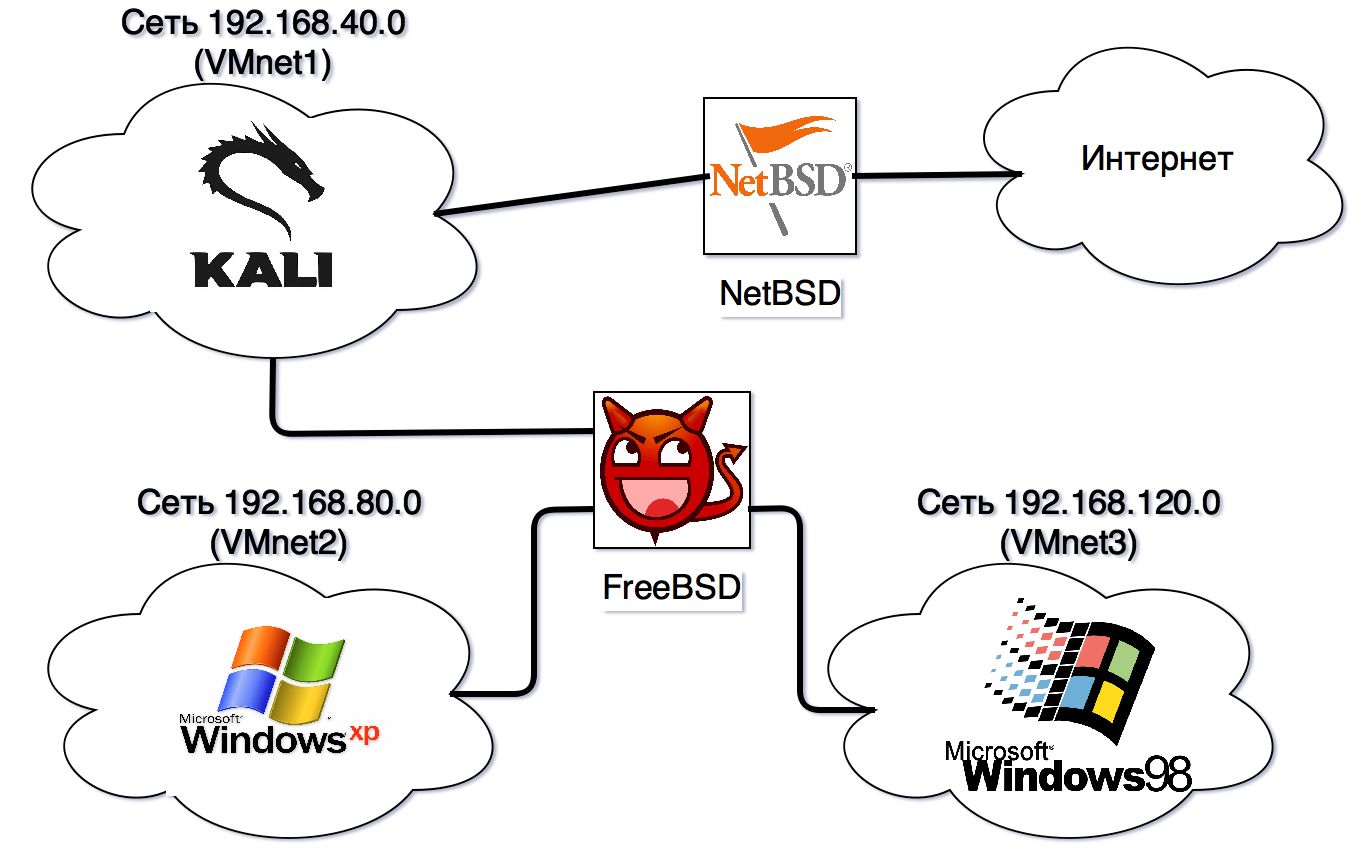
\includegraphics[width=\textwidth]{img/KKS_simple}
\end{center}
\end{frame}

\begin{frame}
\frametitle{Сведения о виртуальных системах}
С помощью средств \textbf{VMware} были созданы виртуальная машины, с использованием ниже представленных операционных систем, с соответствующим выделением оперативной памяти.
\tabulinesep = 1mm
\begin{longtabu} to \textwidth {|X[ c , m ] |X[2, c , m ] | X[ c , m ]|}\firsthline\hline
\textbf{Название}&\textbf{Версия}&\textbf{Объем RAM}\\ \hline \endfirsthead
NetBSD&7.1.1 64-bit x86&256 MB\\ \hline
FreeBSD&11.1-RELEASE 64-bit x86&256 MB\\ \hline
Kali Linux&2017.2 64-bit x86&1.5 GB\\ \hline
Windows XP Professional&5.1.2600 SP3 Сборка 2600&512 MB\\ \hline
Windows 98&4.10.2222A&256 MB\\ \hline
\end{longtabu}

\end{frame}

\begin{frame}
\frametitle{Структура сети}
\begin{itemize}
\item Каждый представитель подсетей (VMnet1, Vmnet2, VMnet3) имеет один сетевой адаптер, шлюз – два, а маршрутизатор – три сетевых адаптера.
\item Хост Win98 имеет статический адрес 192.168.120.15, хост Kali Linux также имеет статический адрес 192.168.40.32, а хост WinXP получает адрес 192.168.80.128 динамически с помощью виртуального сервера DHCP.
\end{itemize}
\tabulinesep = 1mm
\begin{longtabu} to \textwidth {|X[ c , m ] |X[ c , m ] | X[2, c , m ]|X[c , m ]|}\firsthline\hline

\textbf{Название сети}&\textbf{Адрес сети}&\textbf{Подключенные узлы}&\textbf{DHCP}\\ \hline \endfirsthead
	
VMnet1&192.168.40.0&Kali Linux, NetBSD, FreeBSD&\xmark\\ \hline
VMnet2&192.168.80.0&FreeBSD, Windows XP&\cmark\\ \hline
VMnet3&192.168.120.0&FreeBSD, Windows 98&\xmark\\ \hline
VMnet4&192.168.32.0&NetBSD&\cmark\\ \hline

\end{longtabu}
\end{frame}

\begin{frame}
\frametitle{Структура сети}
\begin{itemize}
\item  Для простоты, адресам всех сетевых адаптеров маршрутизатора назначены одинаковые суффиксы – 192.168.40.2 (для связи с сетью VMnet1), 192.168.80.2 (для связи с сетью VMnet2), 192.168.120.2 (для связи с сетью VMnet3)
\item Функциональное назначение шлюза (обеспечение взаимодействия ККС с внешними сетями) предполагает наличие какого-нибудь механизма сопряжения IP-адресов. Таким механизмом является служба NAT (преобразование сетевых адресов), подключённая к вспомогательной сети VMnet4, в которую (кроме устройства NAT) входит DHCP-сервер и шлюз.
\item Адрес «внешнего» сетевого адаптера шлюза назначается динамически (DHCP-сервером сети VMnet4) – 192.168.32.128, а адрес «внутреннего» сетевого адаптера шлюза (входящего в сеть VMnet1) статически – 192.168.40.57.
\end{itemize}

\end{frame}

\begin{frame}
\frametitle{Схема компьютерной сети}
\begin{center}  
	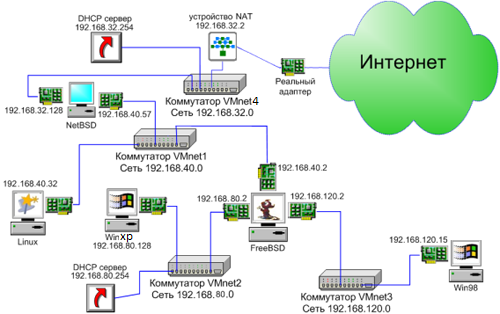
\includegraphics[width=\textwidth]{img/KKS_full}
\end{center}
\end{frame}

\section{Создание сетей}

\begin{frame}
\frametitle{Создание VMnet1}
\begin{center}  
	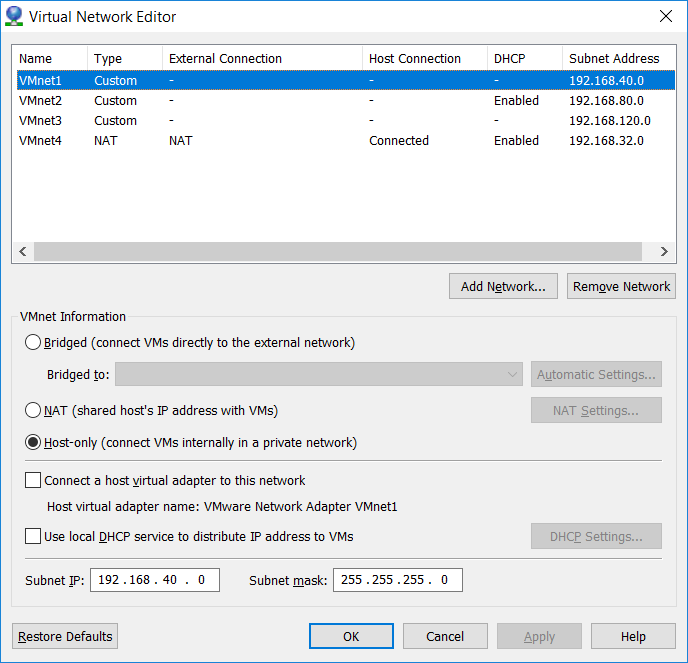
\includegraphics[width=.72\textwidth]{img/vmnet_1}
\end{center}
\end{frame}

\begin{frame}
\frametitle{Создание VMnet2}
\begin{center}  
	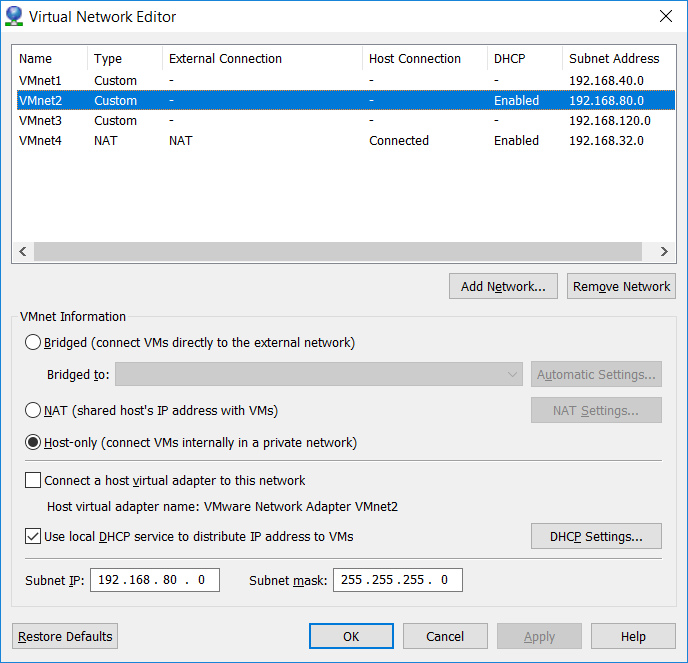
\includegraphics[width=.72\textwidth]{img/vmnet_2}
\end{center}
\end{frame}

\begin{frame}
\frametitle{Создание VMnet3}
\begin{center}  
	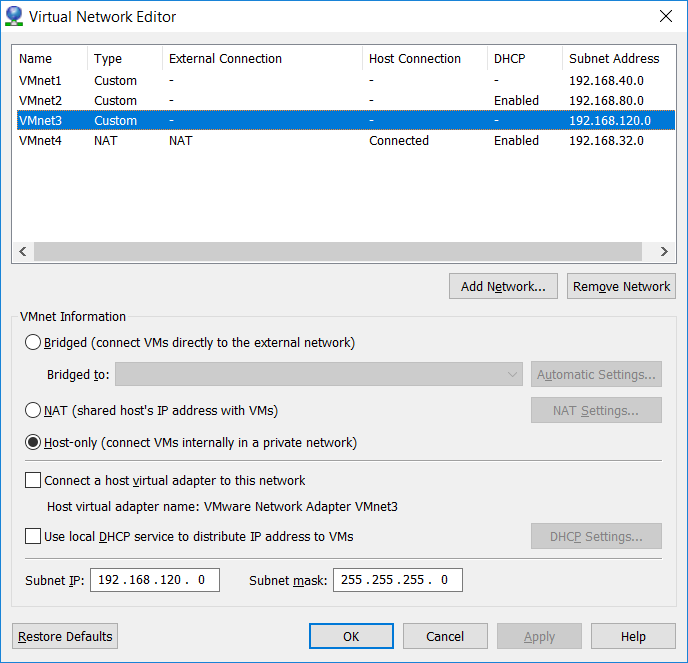
\includegraphics[width=.72\textwidth]{img/vmnet_3}
\end{center}
\end{frame}

\begin{frame}
\frametitle{Создание VMnet4}
\begin{center}  
	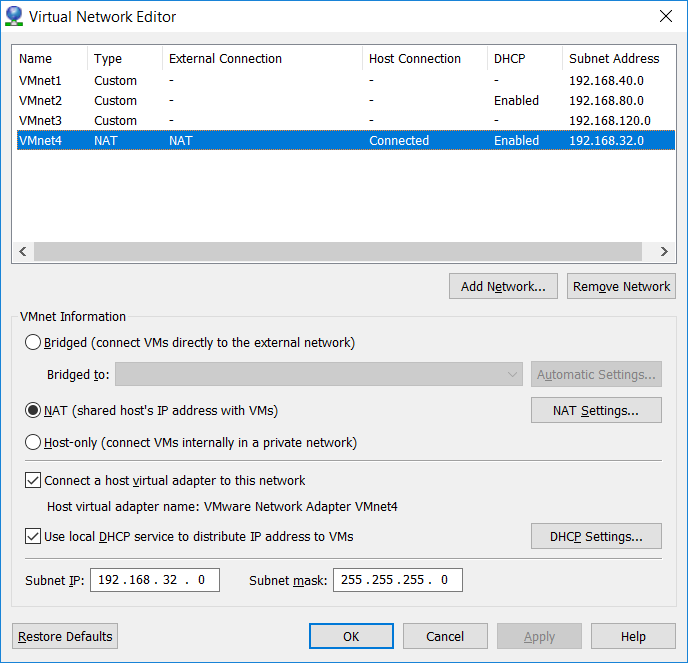
\includegraphics[width=.72\textwidth]{img/vmnet_4}
\end{center}
\end{frame}
		
\section{Конфигурация сетевых интерфейсов}

\begin{frame}
\frametitle{Настройка Windows 98}
\begin{center}  
	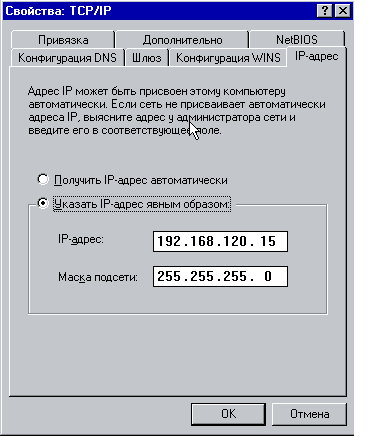
\includegraphics[width=.51\textwidth]{img/win98_1}
	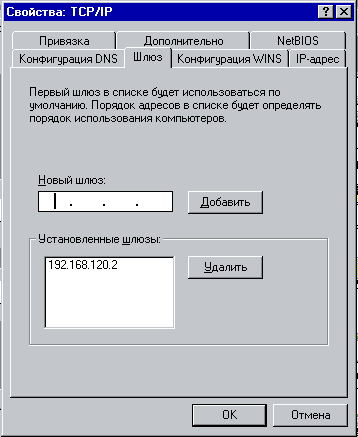
\includegraphics[width=.48\textwidth]{img/win98_2}
\end{center}
\end{frame}

\begin{frame}
\frametitle{Настройка Windows XP}
\begin{center}  
	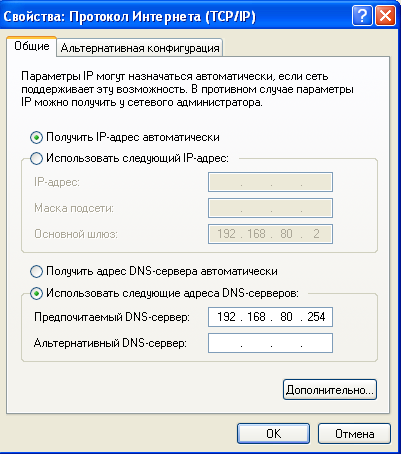
\includegraphics[width=.52\textwidth]{img/winXp_1}
	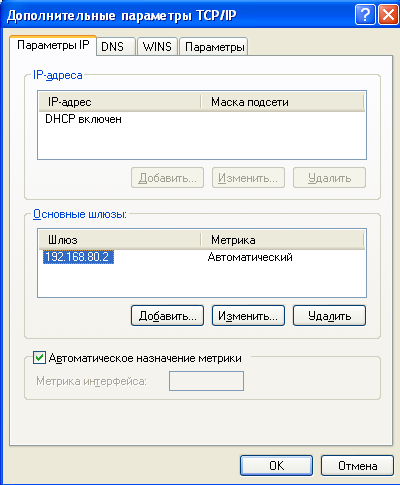
\includegraphics[width=.47\textwidth]{img/winXp_2}
\end{center}
\end{frame}

\begin{frame}
\frametitle{Настройка Kali Linux}
\begin{center}  
	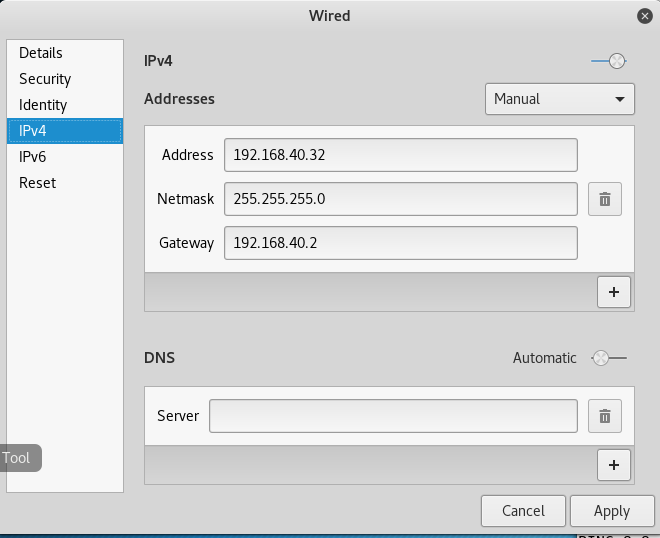
\includegraphics[width=.85\textwidth]{img/kali_1}
\end{center}
\end{frame}

\begin{frame}[fragile]
\frametitle{Настройка NetBSD}
\begin{enumerate}
\item Узнать названия сетевых адаптеров с помощью команды ifconfig, в моем случае это pcn0, pcn1.
\item Разрешаем ip forwarding добавляя в файл \textbf{/etc/sysctl.conf}:
\begin{lstlisting}[language={}]
net.inet.ip.forwarding=1
\end{lstlisting}
\item Внести следующие настройки в файл \textbf{/etc/rc.conf}:
\begin{enumerate}
\item Указание шлюза по умолчанию:
\begin{lstlisting}[language={}]
defaultroute=192.168.32.2
\end{lstlisting}
\item Задаем ip адрес и сетевую маску для одного из интерфейсов:
\begin{lstlisting}[language={}]
ifconfig_pcn0="inet 192.168.40.57 netmask 255.255.255.0"
\end{lstlisting}
\item Разрешаем настройку по DHCP.
\begin{lstlisting}[language={}]
dhclient=yes	
dhclient_flags=pcn1
ifconfig_pcn1=DHCP
\end{lstlisting}
\item Разрешаем запуск NAT:
\begin{lstlisting}[language={}]
ipnat=yes
\end{lstlisting}
\end{enumerate}
\end{enumerate}
\end{frame}

\begin{frame}[fragile]
\frametitle{Настройка NetBSD}
\begin{enumerate}
\setcounter{enumi}{3}
\item Задаем правила NAT в файле /etc/ipnat.conf:
\begin{lstlisting}[language={}]
map pcn1 192.168.40.0/24 -> 0/32 portmap tcp/udp 40000:60000
map pcn1 192.168.40.0/24 -> 0/32
\end{lstlisting}
\item В консоли прописываем следующие команды:
\begin{lstlisting}[language={}]
route add -net 192.168.80.0 -netmask 255.255.255.0 192.168.40.2
route add -net 192.168.120.0 -netmask 255.255.255.0 192.168.40.2
\end{lstlisting}
Так как например Windows 98 находится в другом широковещательном домене, были добавлены маршруты, чтобы NetBSD знала куда отвечать.
\end{enumerate}
\end{frame}


\begin{frame}[fragile]
\frametitle{Настройка FreeBSD}
\begin{enumerate}
\item Узнать названия сетевых адаптеров с помощью команды ifconfig, в моем случае это em0, em1, em2.
\item Внести следующие настройки в файл \textbf{/etc/rc.conf}:
\begin{lstlisting}[language={}]
gateway_enable="YES"
\end{lstlisting}
\begin{enumerate}
\item Разрешаем ip forwarding при помощи команды:
\begin{lstlisting}[language={}]
defaultrouter=192.168.40.57
\end{lstlisting}
\item Задаем ip адрес и сетевую маску для всех интерфейсов:
\begin{lstlisting}[language={}]
ifconfig_em0=inet 192.168.40.2 netmask 255.255.255.0
ifconfig_em1=inet 192.168.80.2 netmask 255.255.255.0
ifconfig_em2=inet 192.168.120.2 netmask 255.255.255.0
\end{lstlisting}
\item Разрешаем запуск NAT:
\begin{lstlisting}[language={}]
ipnat_enable="YES"
\end{lstlisting}
\end{enumerate}
\end{enumerate}
\end{frame}

\begin{frame}[fragile]
\frametitle{Настройка FreeBSD}
\begin{enumerate}
\setcounter{enumi}{2}
\item После этого необходимо задать правила NAT для сопряжения адресов. Это делается путем редактирования файла \textbf{/etc/ipnat.rules}:
\begin{lstlisting}[language={}]
map em0 192.168.80.0/24 -> 0.0.0.0/32 portmap tcp/udp 40000:60000 
map em0 192.168.80.0/24 -> 0.0.0.0/32 
map em0 192.168.120.0/24 -> 0.0.0.0/32 portmap tcp/udp 40000:60000
map em0 192.168.120.0/24 -> 0.0.0.0/32
\end{lstlisting}
Эти строки позволяет корректно обрабатывать tcp, udp, icmp пакеты.
\end{enumerate}
\end{frame}

\section{Тестирование сети}

\begin{frame}[fragile]
\frametitle{Тестирование NetBSD}
\begin{center}  
	\fbox{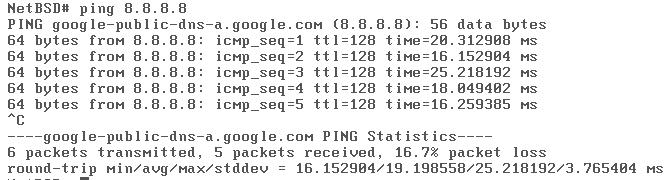
\includegraphics[width=\textwidth]{img/testing_netbsd}}
\end{center}
\end{frame}

\begin{frame}[fragile]
\frametitle{Тестирование Kali Linux}
\begin{center}  
	\fbox{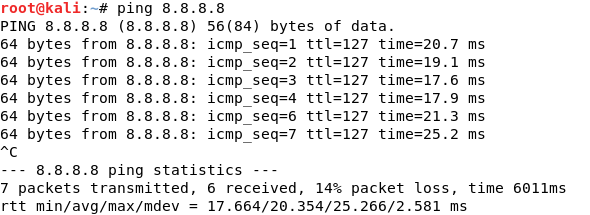
\includegraphics[width=\textwidth]{img/testing_kali}}
\end{center}
\end{frame}

\begin{frame}[fragile]
\frametitle{Тестирование FreeBSD}
\begin{center}  
	\fbox{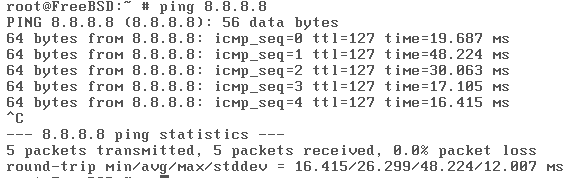
\includegraphics[width=\textwidth]{img/testing_freebsd}}
\end{center}
\end{frame}

\begin{frame}[fragile]
\frametitle{Тестирование Windows XP}
\begin{center}  
	\fbox{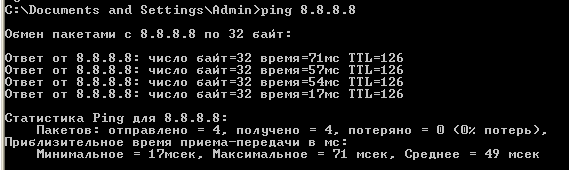
\includegraphics[width=\textwidth]{img/testing_winxp}}
\end{center}
\end{frame}

\begin{frame}[fragile]
\frametitle{Тестирование Windows 98}
\begin{center}  
	\fbox{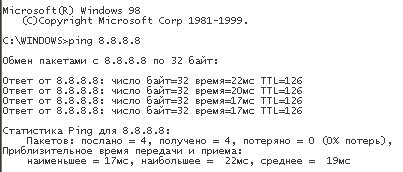
\includegraphics[width=\textwidth]{img/testing_win98}}
\end{center}
\end{frame}

\begin{frame}[fragile]
\frametitle{Вывод}
В данной работе была рассмотрена эмуляция корпоративной компьютерной сети(ККС), которая содержит три основных и один вспомогательный сегмент сети. Средствами VMWare были созданы:
\begin{itemize}
\item Виртуальные машины, с различными представителями операционных систем.
\item Виртуальные сети(с различными параметрами).
\item Адаптеры для виртуальных машин.
\end{itemize}
Это позволило эмулировать заданную ККС, в которой использовались:
\begin{itemize}
\item Статическая адресация;
\item Динамическое выделение IP адреса;
\item Статическая и динамическая маршрутизация.
\end{itemize}
Также имелась возможность выхода в сеть "Интернет" из каждой операционной системы.
\end{frame}	
	

	
\end{document}